\documentclass{report}
% Include all project wide packages here.
\usepackage{fullpage}
\usepackage[style=ieee]{biblatex}
\usepackage[dutch]{babel}

\renewcommand{\familydefault}{\sfdefault}

\setmainfont[Ligatures=TeX]{Myriad Pro}
\setmathfont{Asana Math}
\setmonofont{Lucida Console}

\usepackage{titlesec, blindtext, color}
\definecolor{gray75}{gray}{0.75}
\newcommand{\hsp}{\hspace{20pt}}
\titleformat{\chapter}[hang]{\Huge\bfseries}{\thechapter\hsp\textcolor{gray75}{|}\hsp}{0pt}{\Huge\bfseries}
\renewcommand{\familydefault}{\sfdefault}
\renewcommand{\arraystretch}{1.2}
\setlength\parindent{0pt}

%For code listings
\definecolor{black}{rgb}{0,0,0}
\definecolor{browntags}{rgb}{0.65,0.1,0.1}
\definecolor{bluestrings}{rgb}{0,0,1}
\definecolor{graycomments}{rgb}{0.4,0.4,0.4}
\definecolor{redkeywords}{rgb}{1,0,0}
\definecolor{bluekeywords}{rgb}{0.13,0.13,0.8}
\definecolor{greencomments}{rgb}{0,0.5,0}
\definecolor{redstrings}{rgb}{0.9,0,0}
\definecolor{purpleidentifiers}{rgb}{0.01,0,0.01}


\lstdefinestyle{csharp}{
language=[Sharp]C,
showspaces=false,
showtabs=false,
breaklines=true,
showstringspaces=false,
breakatwhitespace=true,
escapeinside={(*@}{@*)},
columns=fullflexible,
commentstyle=\color{greencomments},
keywordstyle=\color{bluekeywords}\bfseries,
stringstyle=\color{redstrings},
identifierstyle=\color{purpleidentifiers},
basicstyle=\ttfamily\small}

\lstdefinestyle{c}{
language=C,
showspaces=false,
showtabs=false,
breaklines=true,
showstringspaces=false,
breakatwhitespace=true,
escapeinside={(*@}{@*)},
columns=fullflexible,
commentstyle=\color{greencomments},
keywordstyle=\color{bluekeywords}\bfseries,
stringstyle=\color{bluestrings},
identifierstyle=\color{purpleidentifiers}
}

\lstdefinestyle{vhdl}{
language=VHDL,
showspaces=false,
showtabs=false,
breaklines=true,
showstringspaces=false,
breakatwhitespace=true,
escapeinside={(*@}{@*)},
columns=fullflexible,
commentstyle=\color{greencomments},
keywordstyle=\color{bluekeywords}\bfseries,
stringstyle=\color{redstrings},
identifierstyle=\color{purpleidentifiers}
}

\lstdefinestyle{xaml}{
language=XML,
showspaces=false,
showtabs=false,
breaklines=true,
showstringspaces=false,
breakatwhitespace=true,
escapeinside={(*@}{@*)},
columns=fullflexible,
commentstyle=\color{greencomments},
keywordstyle=\color{redkeywords},
stringstyle=\color{bluestrings},
tagstyle=\color{browntags},
morestring=[b]",
  morecomment=[s]{<?}{?>},
  morekeywords={xmlns,version,typex:AsyncRecords,x:Arguments,x:Boolean,x:Byte,x:Char,x:Class,x:ClassAttributes,x:ClassModifier,x:Code,x:ConnectionId,x:Decimal,x:Double,x:FactoryMethod,x:FieldModifier,x:Int16,x:Int32,x:Int64,x:Key,x:Members,x:Name,x:Object,x:Property,x:Shared,x:Single,x:String,x:Subclass,x:SynchronousMode,x:TimeSpan,x:TypeArguments,x:Uid,x:Uri,x:XData,Grid.Column,Grid.ColumnSpan,Click,ClipToBounds,Content,DropDownOpened,FontSize,Foreground,Header,Height,HorizontalAlignment,HorizontalContentAlignment,IsCancel,IsDefault,IsEnabled,IsSelected,Margin,MinHeight,MinWidth,Padding,SnapsToDevicePixels,Target,TextWrapping,Title,VerticalAlignment,VerticalContentAlignment,Width,WindowStartupLocation,Binding,Mode,OneWay,xmlns:x}
}

%defaults
\lstset{
basicstyle=\ttfamily\small,
extendedchars=false,
numbers=left,
numberstyle=\ttfamily\tiny,
stepnumber=1,
tabsize=4,
numbersep=5pt
}
\addbibresource{../../library/bibliography.bib}

\title{EPO-2: Mid-term Design Report - Bijlagen}
\author{Robin Hes \and Erwin de Haan}

\begin{document}

\chapter{Bijlagen}
\label{ch:bijlagen}

\newpage
\section{Plan van aanpak}
\label{sec:pva}

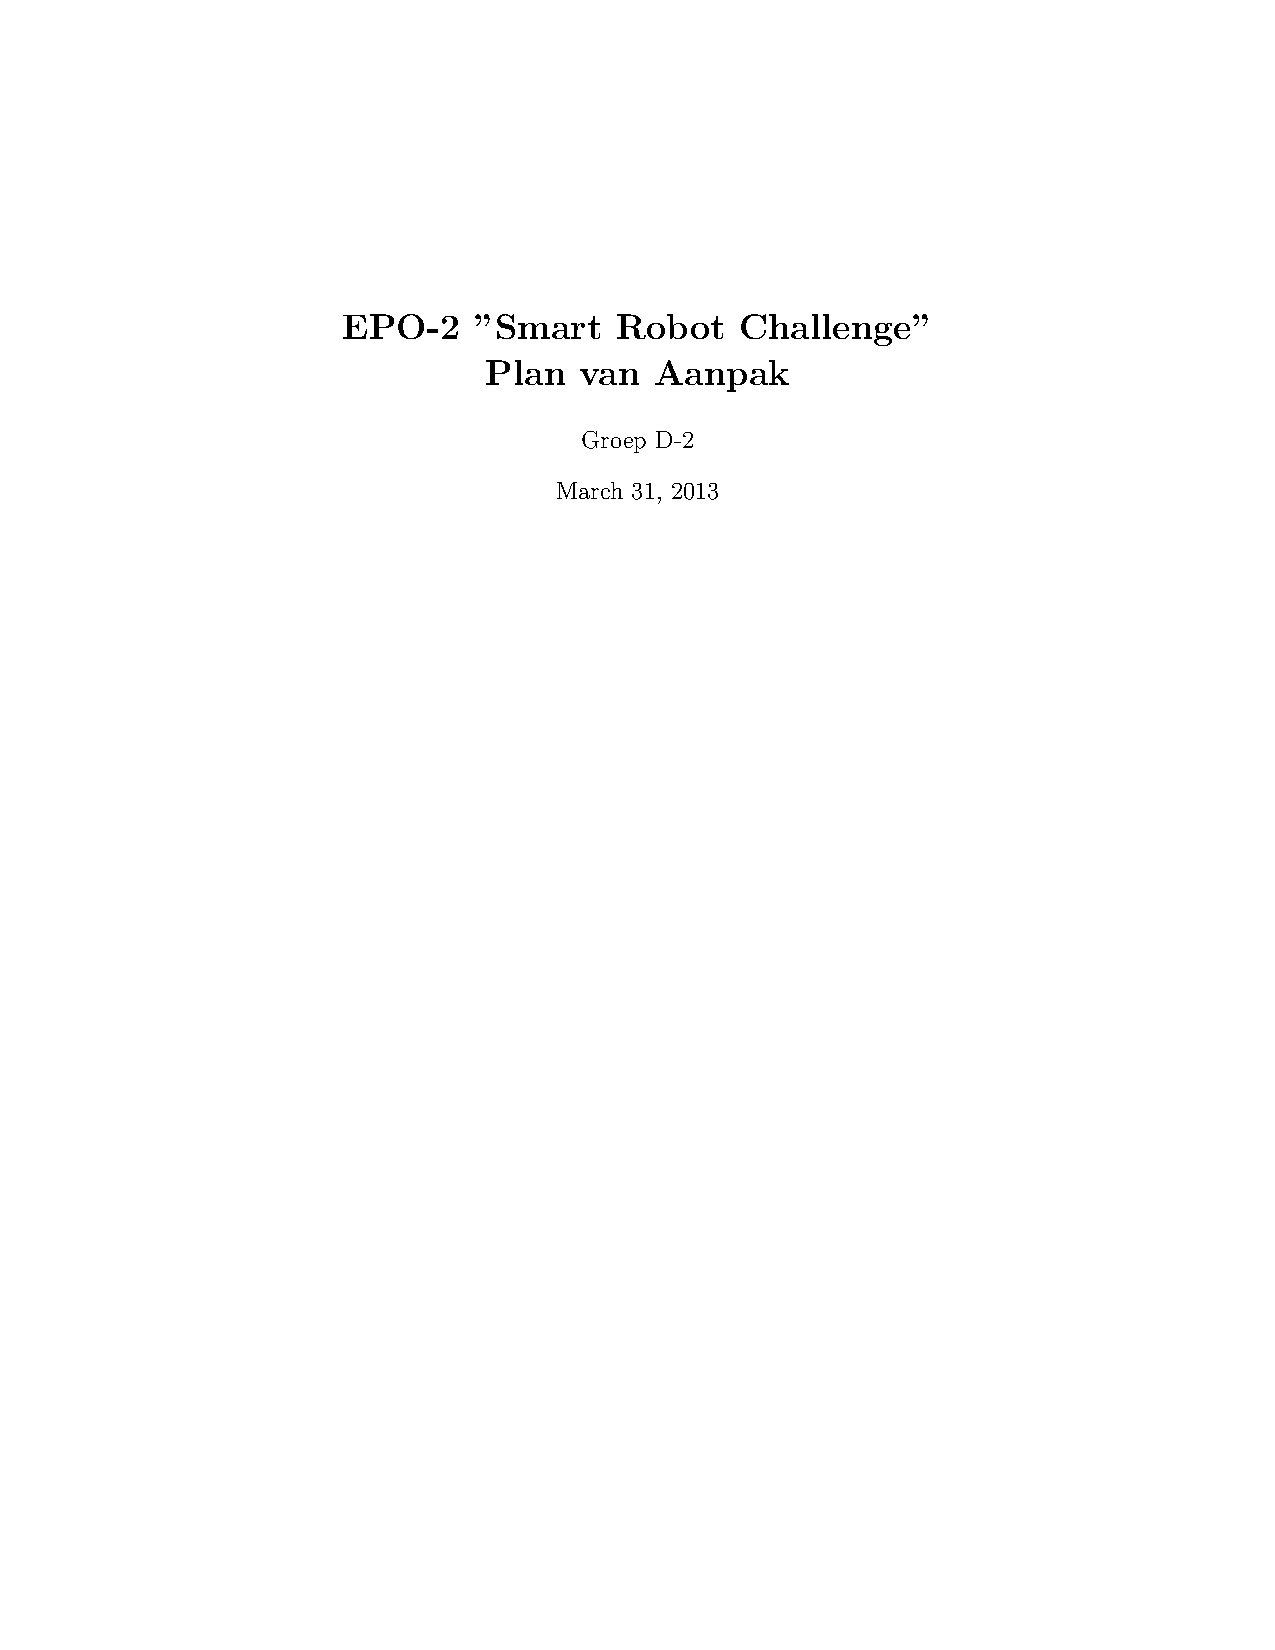
\includepdf[pages={1-10}]{plan-van-aanpak-rc.pdf}

\section{Routeplanner Pseudocode}
\label{sec:pseudocode}

\subsection{Lee}
\label{ssec:pseudocode-lee}
\cite{pseudocode-lee}

\subsection{A*}
\label{ssec:pseudocode-astar}
\cite{pseudocode-astar}

\newpage
\section{Communicatie}
\label{sec:communicatie}
\begin{table}[H]
\centering
\caption{}
\begin{subtable}{0.48\textwidth}
\subcaption{Protocol Rev. F}
\label{tab:comProtocol}
\centering
\begin{tabular}{@{}lll@{}}
\toprule
\textbf{Commando} & \textbf{hex} & \textbf{2-way} \\
\midrule
Forward				& 0x46 	& to robot only\\
Stop 					& 0x53 	& to robot only\\
Right 					& 0x52 	& to robot only\\
Left 					& 0x4C 	& to robot only\\
Turn					& 0x54 	& to robot only\\
Back					& 0x42 	& to robot only\\
Continue				& 0x01	& to robot only\\
Done 					& 0x04	& to robot only\\
Acknowledge 			& 0x06	& both ways\\
Negative Acknowledge 		& 0x15	& both ways \\
Enquiry 				& 0x05	& to pc only\\
Mine 					& 0x07	& to pc only\\
Half					& 0x86 	& to pc only\\
Unknown 				& 0x00	& both ways\\
\bottomrule
\end{tabular}
\end{subtable}
\quad
\begin{subtable}{0.48\textwidth}
\subcaption{XBee Settings van de twee modules. Master is de Robot.}
\label{tab:XBeeSettings}
\centering
\begin{tabular}{@{}ccc@{}}
\toprule
\textbf{Setting} & \textbf{master}& \textbf{slave} \\
\midrule
Channel				& 0x1A 	& 0x1A\\
Pan ID				& 0x1337 	& 0x1337\\
Destination High			& 0x0000	& 0x0000\\
Destination Low			& 0x8564 	& 0x4658\\
My Address				& 0x4658 	& 0x8564\\
*		 			& (default)	&(default)\\
\bottomrule
\end{tabular}
\end{subtable}
\end{table}
\section{Finite State Machines}
\label{sec:statemachines}
\begin{figure}[H]
\centering
\caption{De FSM's op de FPGA}
\begin{subfigure}{0.40\linewidth}
\subcaption{FSM van de receiver.}
\label{fig:fsmReceiver}
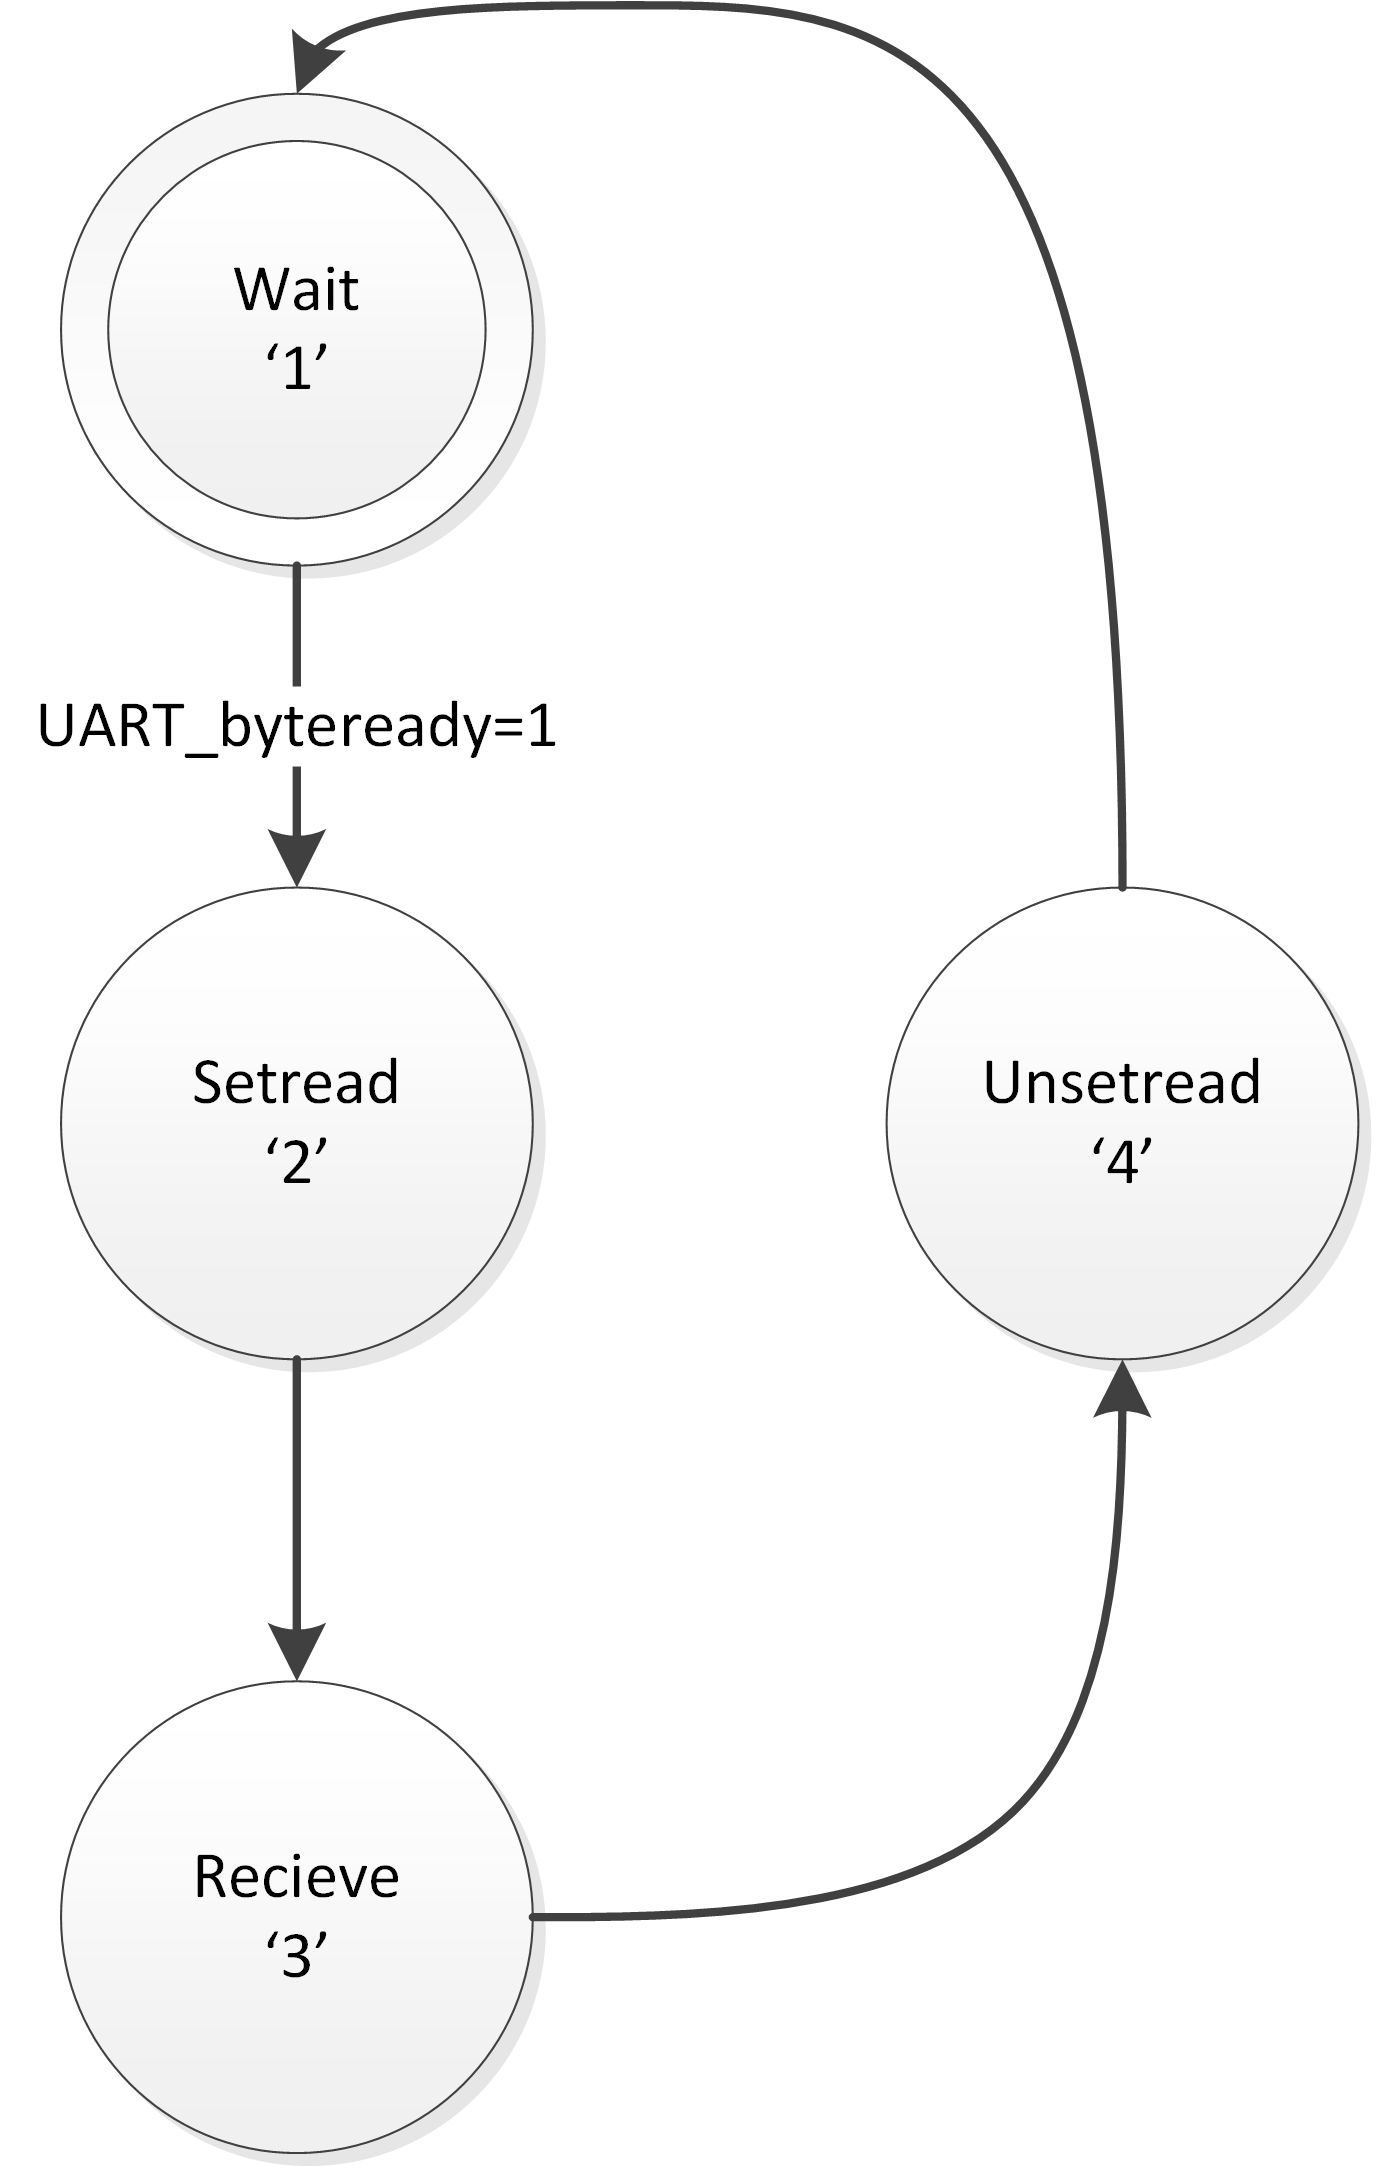
\includegraphics[width=\linewidth]{FSMReceiver}
\end{subfigure}
\quad
\begin{subfigure}{0.40\linewidth}
\subcaption{FSM van de sender.}
\label{fig:fsmSender}
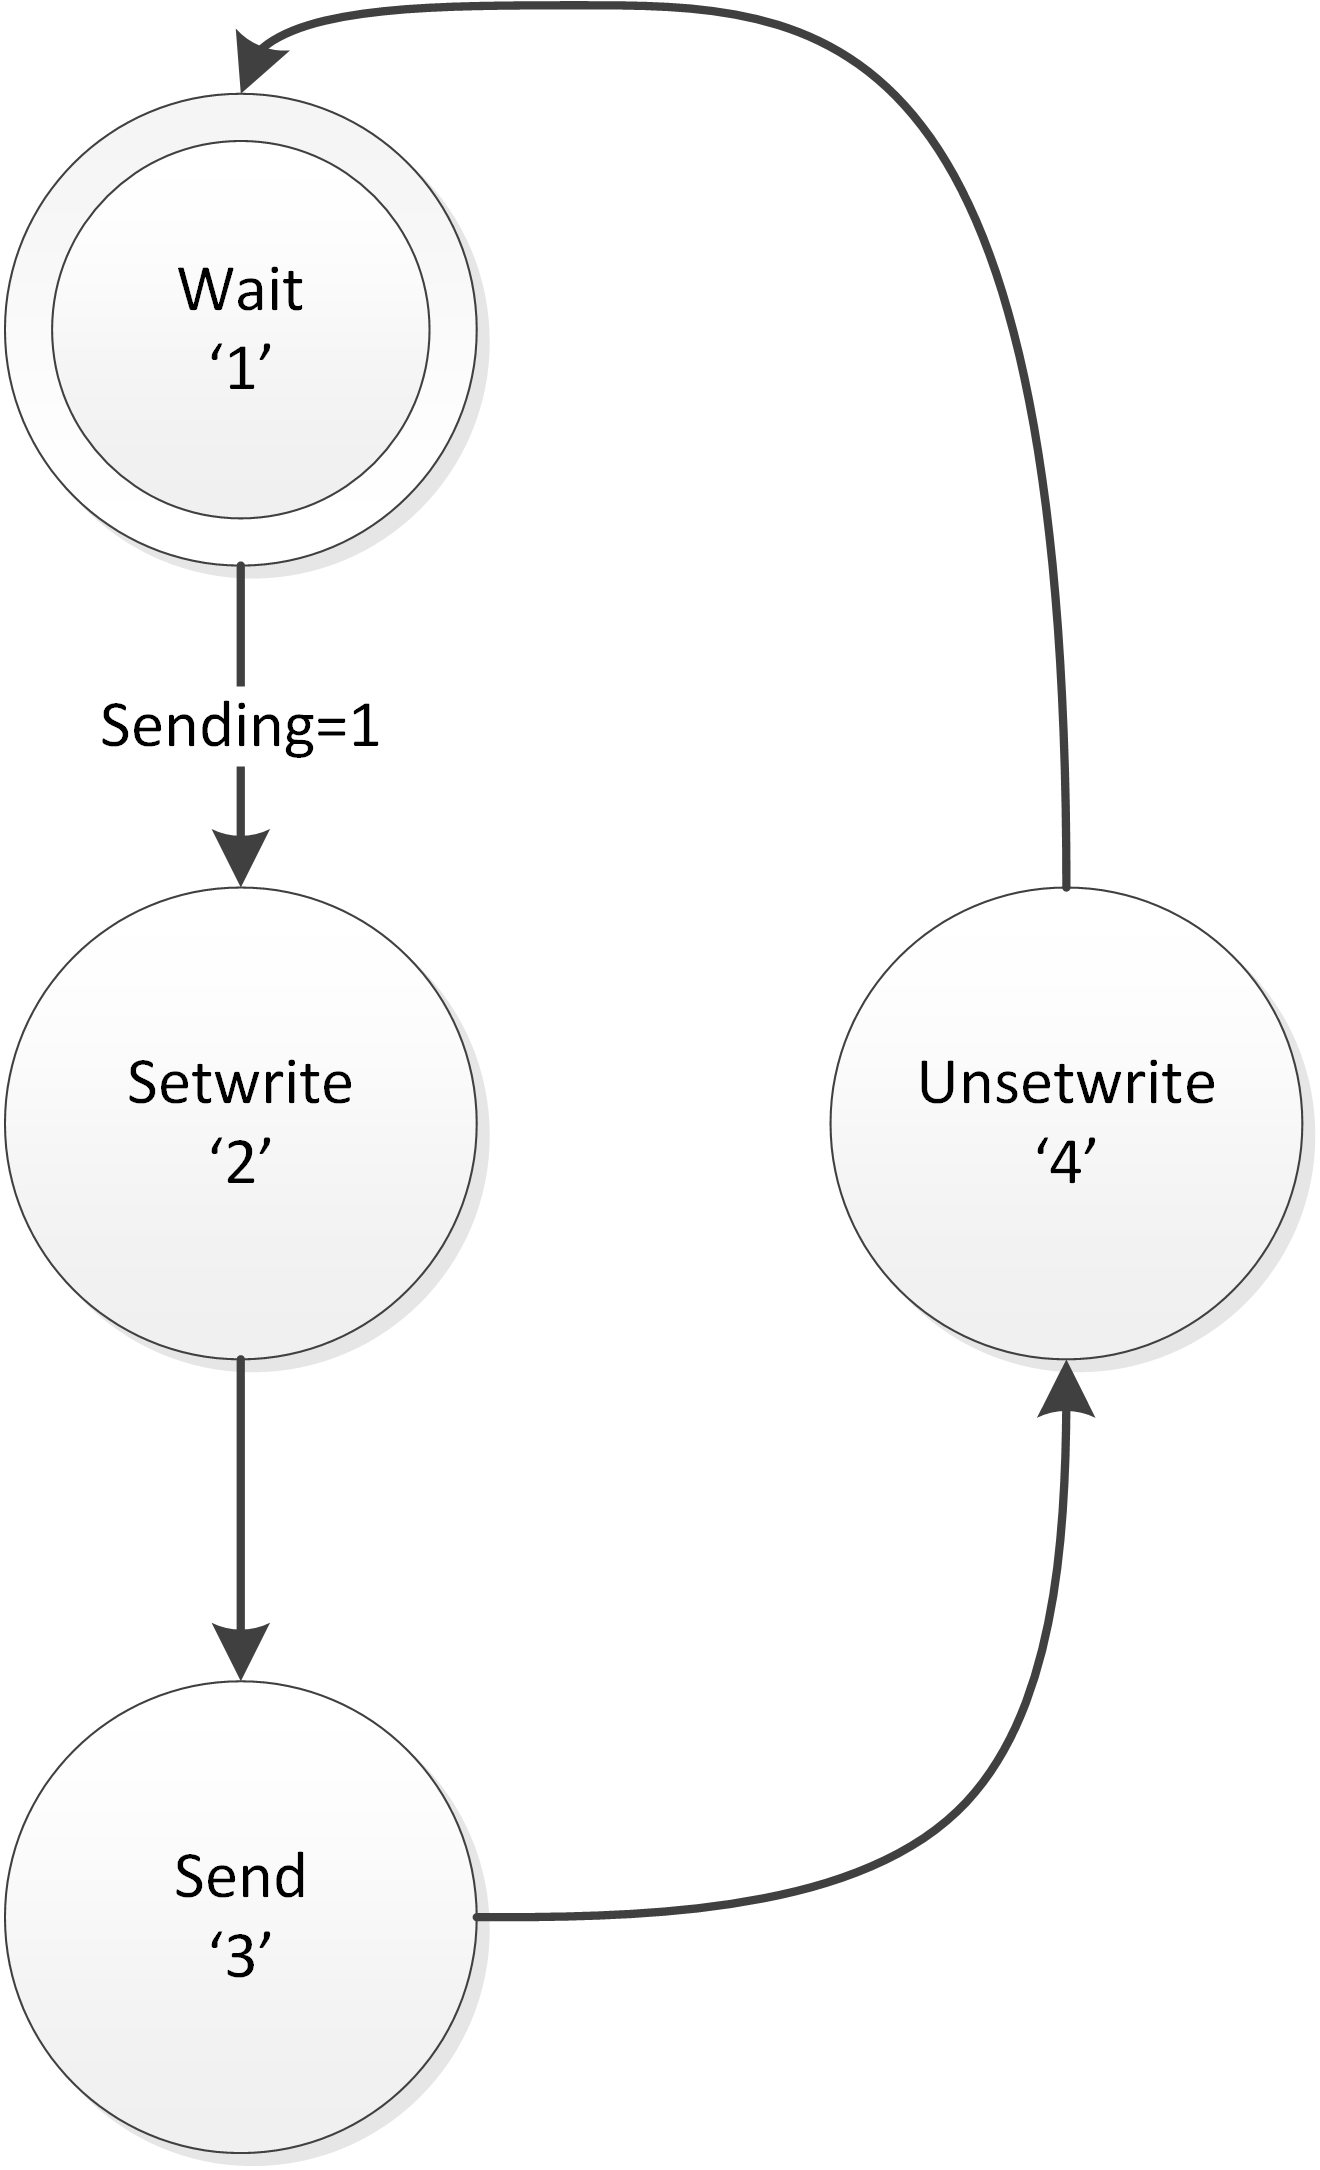
\includegraphics[width=\linewidth]{FSMSender}
\end{subfigure}
\end{figure}

\begin{figure}[H]
\caption{FSM van het hoofd systeem.}
\label{fig:fsmMain}
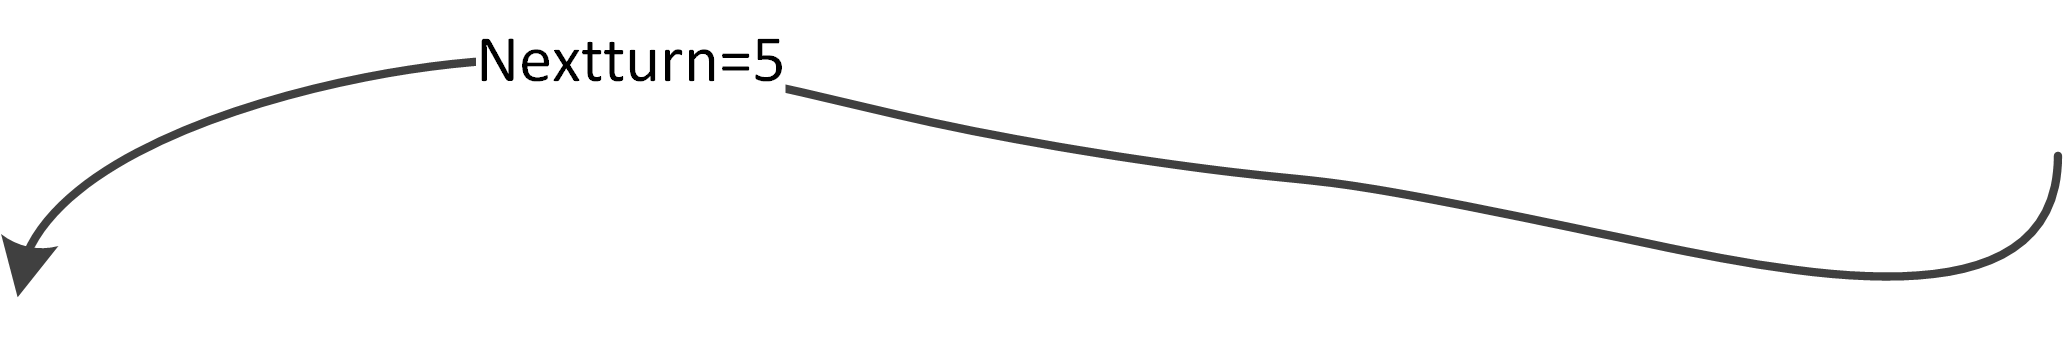
\includegraphics[width=0.8\linewidth]{FSMMain}
\end{figure}

\section{Broncode}
\subimport{../../../}{sourceBijlage}
\end{document}